\begin{figure}[t]

    \begin{subfigure}[t]{0.48\textwidth}
        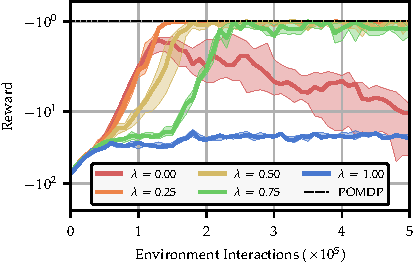
\includegraphics[width=0.95\textwidth]{figures/OSC/lambda_sweep/lam_sweep_results_TigerDoor_True_tests_results_AdaptAsymDagger_cr_logs_lam_sweep_4_.pdf}
        \caption{Reward.}
        \label{fig:osc:lambda:reward}
    \end{subfigure}%
    %
    \hfill%
    %
    \begin{subfigure}[t]{0.48\textwidth}
        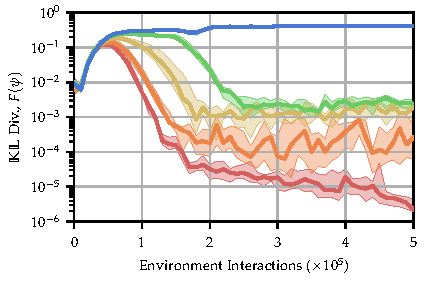
\includegraphics[width=0.95\textwidth]{figures/OSC/lambda_sweep/lam_sweep_divergence_TigerDoor_True_tests_results_AdaptAsymDagger_cr_logs_lam_sweep_4_.pdf}
        \caption{Divergence.}
        \label{fig:osc:lambda:divergence}
    \end{subfigure}%
    \vspace{-0.25cm}
    \caption{Results showing the affect of the GAE parameter $\lambda$ on A2D, applied to the  Tiger Door 2 environment.  The reward is normalized such that the optimal reward under the POMDP is $-10^{0}$.  As predicted, we see that lower $\lambda$ values yield faster convergence and monotonically lower policy divergences.  However, as this is equivalent to TD0, the RL is unstable (obscured in this plot are short, sharp drops in the reward and rises in the divergence).  Eventually, all traces begin to diverge from the optimal policy.  For any $\lambda$ value less than unity, convergence is stable (and the short, sharp drops do not exist).  Finally, and again as predicted, we see that learning does not converge when $\lambda = 1$, with reward remaining flat and low, and the divergence remaining high. { }%
    }
    \label{fig:osc:lambda}
\end{figure}
